\documentclass{beamer}

\usepackage{url}

\newcommand\vs{\vspace{\baselineskip}}

\newcommand\titlecite{
{\em Of all natural systems, living matter preserves inscribed in its organization the largest amount of its own past history .... no other system is better}
 aufgehoben:
{\em constantly abolished and simultaneously preserved.}
\cite{PaulingZuckerkandl63}}

\newcommand\presentation[1]{ \section*{PRESENTATION: #1} }



% workaround for beamer bug
\providecommand\thispdfpagelabel[1]{}  % workaround

% presentation
\mode<presentation>
{
  \usetheme{Warsaw}
  % or ...

  \setbeamercovered{transparent}
  % or whatever (possibly just delete it)
}


\usepackage[english]{babel}
% or whatever

\usepackage[latin1]{inputenc}
% or whatever

\usepackage{times}
\usepackage[T1]{fontenc}
% Or whatever. Note that the encoding and the font should match. If T1
% does not look nice, try deleting the line with the fontenc.


\title[Compression] % (optional, use only with long paper titles)
{Data compression}

\subtitle
{Probabilistic models} % (optional)

\author% [Holmes] (optional, use only with lots of authors)
{I.~Holmes} % \inst{1} \and S.~Another\inst{2}
% - Use the \inst{?} command only if the authors have different
%   affiliation.

\institute[University of California, Berkeley] % (optional, but mostly needed)
{
%  \inst{1}%
  Department of Bioengineering\\
  University of California, Berkeley}
% - Use the \inst command only if there are several affiliations.
% - Keep it simple, no one is interested in your street address.

\date%[Short Occasion] % (optional)
{Spring semester}

\subject{Talks}
% This is only inserted into the PDF information catalog. Can be left
% out. 



% If you have a file called "university-logo-filename.xxx", where xxx
% is a graphic format that can be processed by latex or pdflatex,
% resp., then you can add a logo as follows:

% \pgfdeclareimage[height=0.5cm]{university-logo}{university-logo-filename}
% \logo{\pgfuseimage{university-logo}}



% Delete this, if you do not want the table of contents to pop up at
% the beginning of each subsection:
\AtBeginSubsection[]
{
  \begin{frame}<beamer>{Outline}
    \tableofcontents[currentsection,currentsubsection]
  \end{frame}
}


% If you wish to uncover everything in a step-wise fashion, uncomment
% the following command: 

%\beamerdefaultoverlayspecification{<+->}


\begin{document}

\begin{frame}
  \titlepage
\end{frame}

\begin{frame}{Outline}
  \tableofcontents
  % You might wish to add the option [pausesections]
\end{frame}

\section{Information Theory and Compression}

\begin{frame}{Information-theoretic quantities}

\begin{tabular}{rlcl}
Shannon information: & $h(x)$ & = & $-\log_2 p(x)$ \\
\\
Shannon entropy: & $H_p$ & = & $\expect{h(x)}_p$ \\
\\
Relative entropy: & $D(p||q)$ & = & $\expect{\log \frac{p(x)}{q(x)}}_p$ \\
\\
Mutual information: & $I(x;y)$ & = & $D\left(p(x,y)||p(x)p(y)\right)$ \\
\\
\\
Kolmogorov complexity: & $K({\bf x})$ & = & size of smallest program \\ & & & that outputs ${\bf x}$
\end{tabular}

\end{frame}

\begin{frame}{Theorems}

 \centerline{ 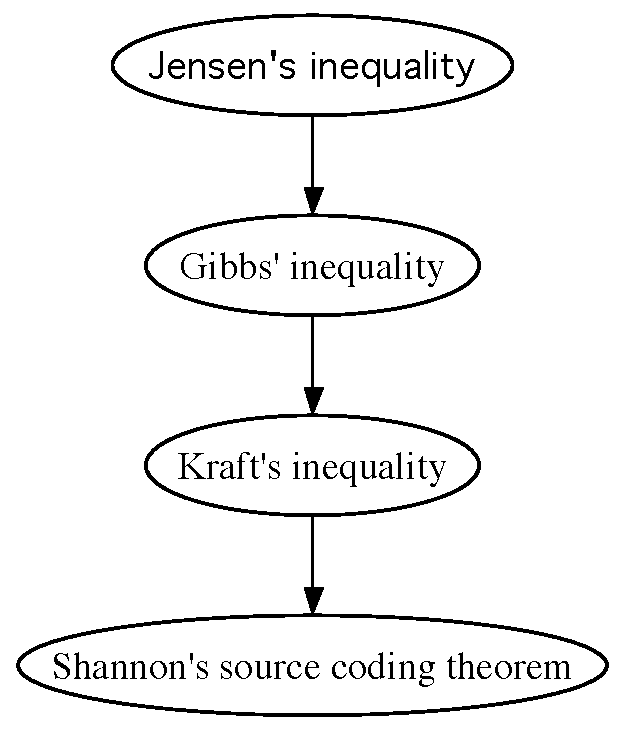
\includegraphics[height=.75\textheight]{theorems-nodates.pdf} }

{\bf Information Theory, Inference and Learning Algorithms.} MacKay (2003)

\end{frame}

\begin{frame}{Jensen's Inequality}

\itemb
  \item A function $f(x)$ is \alert{convex} over $(a,b)$ if every chord lies above the function.
   \inone{$f''(x) \geq 0$ is sufficient.}
  \item Jensen's inequality:
\\
\centerline{\framebox{If $x$ is an rv and $f(x)$ is convex, then $\expect{f(x)} \geq f(\expect{x})$}}
  \item If $f(x)$ is concave, then inequality is reversed.
\iteme

\end{frame}

\begin{frame}{Jensen's Inequality}

\centerline{\framebox{If $x$ is an rv and $f(x)$ is convex, then $\expect{f(x)} \geq f(\expect{x})$}}

\itemb
  \item Physical version:
   \itemb
    \item Let $p(x)$ be $x$-distribution of masses on curve $y=f(x)$.
    \item Then center of gravity $(\expect{x},\expect{f(x)})$ lies above curve.
   \iteme
\iteme

\end{frame}


\begin{frame}{Bounds on the Shannon entropy}


\[
H_p \leq \log |\Omega|
\]

Proof: apply Jensen's inequality to $u=1/p(x)$, $f(u)=-\log u$

\[
\expect{f(u)} \geq f(\expect{u})
\]


\end{frame}

\begin{frame}{Gibbs' Inequality}

\centerline{\framebox{$D(p||q) \geq 0 \quad\quad \mbox{with equality iff $p=q$}$}}

where $p,q$ are probability distributions over the same set $\Omega$, and
\[
D(p||q) = \sum_x p(x) \log \frac{p(x)}{q(x)}
\]
is the \alert{relative entropy} or \alert{Kullback-Leibler divergence}.

Proof: apply Jensen to $u=q(x)/p(x)$, $f(u)=-\log u$

\[
\expect{f(u)} \geq f(\expect{u})
\]

\end{frame}

\begin{frame}{Symbol codes}

\itemb
\item Let $\Omega^+$ be the set of all finite-length strings over $\Omega$
\item A \alert{binary symbol code} $C$ is a mapping from $\Omega$ to $\{0,1\}^+$
\item The \alert{extended code} $C^+$ is a mapping from ${\Omega}^+$ to $\{0,1\}^+$
obtained by concatenating codewords:
\[
       c^+(x_1 x_2 \ldots x_N) = c(x_1)c(x_2)\ldots c(x_N)
\]
\item Side note: it's common to add an \alert{End Of File} symbol to the alphabet, so the decoder knows when to stop
\inone{although it's usually more efficient to send the length of your message first, followed by the symbols}
\iteme

\end{frame}


\begin{frame}{Decodability}

\itemb
\item The code $C$ is \alert{uniquely decodable} if, under the extended code $C^+$,
no two strings have the same encoding.
\item If no codeword is a prefix of any other codeword,
then $C$ is a \alert{prefix code}.
\item All prefix codes are uniquely decodable...
\iteme

\end{frame}

\begin{frame}{Block codes}

\itemb
\item A \alert{block code} is a code over the alphabet $\Omega^N$
\item That is, it divides an $\Omega$-string into blocks of size $N$
\item A common efficiency trick in information theory
 \itemb
 \item e.g. if $|\Omega|=5$, then Shannon info $\sim$2.32 bits/symbol
 \item Naive encoding would require 3 bits/symbol: 0.7 bits/symbol wasted
 \item Block code with $N=3$ requires 7/3 $\simeq$2.33 bits/symbol
 \iteme
\item For any symbol code $C$ there is a trivial block code $C^N$
\iteme

\end{frame}

\section{Theoretical Limits of Compression}

\begin{frame}

\itemb
\item Let $l(x)$ be the length of the codeword $C(x)$
\item Let $p(x)$ be the probability distribution over symbols
\item Define the {\em expected codeword length} of $C$:
\[
L_p(C) = \expect{l(x)}_p
\]
\item \alert{Shannon's Source Coding Theorem} states that
\[
L_p(C) \geq H_p
\]
for any uniquely decodable code $C$.
\item The equality holds if $l(x) = h(x) \quad \forall x$
\iteme

\end{frame}

\begin{frame}{Insight into Source Coding Theorem}

\itemb
\item Given a unique code $C$, is it optimal for anything?
\item Maybe... if there's a distribution $q(x)$ such that $L_q(C) = H_q$
\item This would require that $l(x) = h_q(x) \quad \forall x$, i.e.
\[
q(x) = 2^{-l(x)} / z
\]
where
\[
z = \sum_{x \in {\Omega}} 2^{-l(x)}
\]
is a \alert{partition function}
\item We use these ``implicit probabilities'' to prove the inequality
 \inone{Note that $l(x) = \log(1/q(x)) - \log z$}
\iteme

\end{frame}

\begin{frame}{Partition function for block code}

\itemb
\item Partition function for symbol code $C$ is
\[
z = \sum_{x \in {\Omega}} 2^{-l(x)}
\]
\item Partition function for block code $C^N$ is
\begin{eqnarray*}
z^N & = & \left[ \sum_{x \in {\Omega}} 2^{-l(x)} \right]^N \\
& = & \sum_{x_1 \in {\Omega}} \sum_{x_2 \in {\Omega}} \cdots \sum_{x_N \in {\Omega}} 2^{-(l(x_1)+l(x_2)+\ldots+l(x_N))}
\end{eqnarray*}
\iteme

\end{frame}

\begin{frame}{Rearranging the partition function}

\[
z^N = \sum_{x_1 \in {\Omega}} \sum_{x_2 \in {\Omega}} \cdots \sum_{x_N \in {\Omega}} 2^{-(l(x_1)+l(x_2)+\ldots+l(x_N))}
\]

\itemb
\item The quantity $l(x_1)+l(x_2)+\ldots+l(x_N)$ is the length of the $C^+$-encoding of the string ${\bf x} = x_1 x_2 \cdots x_N$.
\item For every string ${\bf x} \in {\Omega}^N$, there is one term in the above sum for $z^N$.
\item Let
 \itemb
 \item $A_l$ be the number of strings ${\bf x}$ having encoded length $l$
 \item $l_{\mbox{\tiny min}} = \min_x l(x)$
 \item $l_{\mbox{\tiny max}} = \max_x l(x)$
 \iteme
\[
z^N = \sum_{l = Nl_{\mbox{\tiny min}}}^{Nl_{\mbox{\tiny max}}} 2^{-l} A_l
\]
\iteme

\end{frame}

\begin{frame}{The Kraft-McMillan inequality}

\itemb
\item $A_l$ is number of strings with encoded length $l$:
\[
z^N = \sum_{l = Nl_{\mbox{\tiny min}}}^{Nl_{\mbox{\tiny max}}} 2^{-l} A_l
\]
\item If $C$ is uniquely decodable, then $A_l \leq 2^l$. Therefore
\[
z^N = \sum_{l = Nl_{\mbox{\tiny min}}}^{Nl_{\mbox{\tiny max}}} 2^{-l} A_l
\leq \sum_{l = Nl_{\mbox{\tiny min}}}^{Nl_{\mbox{\tiny max}}} 1
\leq Nl_{\mbox{\tiny max}}
\]
\item Since this holds for arbitrarily large $N$, it must be that
\[
z \leq 1
\]
\item This is the \alert{Kraft-McMillan inequality}, now for the source coding theorem
\iteme

\end{frame}

\begin{frame}{Proof of Source Coding Theorem}

\itemb
\item Recall that
\begin{tabular}{rcll}
$L_p(C)$ & = & $\expect{l(x)}_p$ & (definition of $L_p$) \\
$l(x)$ & = & $\log(1/q(x)) - \log z$ & (definition of $q$) \\
$\expect{\log 1/q(x)}_p$ & $\geq$ & $\expect{\log 1/p(x)}_p$ & (Gibbs) \\
$z$ & $\leq$ & 1 & (Kraft-McMillan)
\end{tabular}
\item It follows that
\begin{eqnarray*}
L_p(C) & = & \expect{\log 1/q(x)}_p - \log z \\
& \geq & \expect{\log 1/p(x)}_p - \log z \\
& \geq & H_p
\end{eqnarray*}
\iteme

\end{frame}

\begin{frame}{Theorems (with dates)}

 \centerline{ 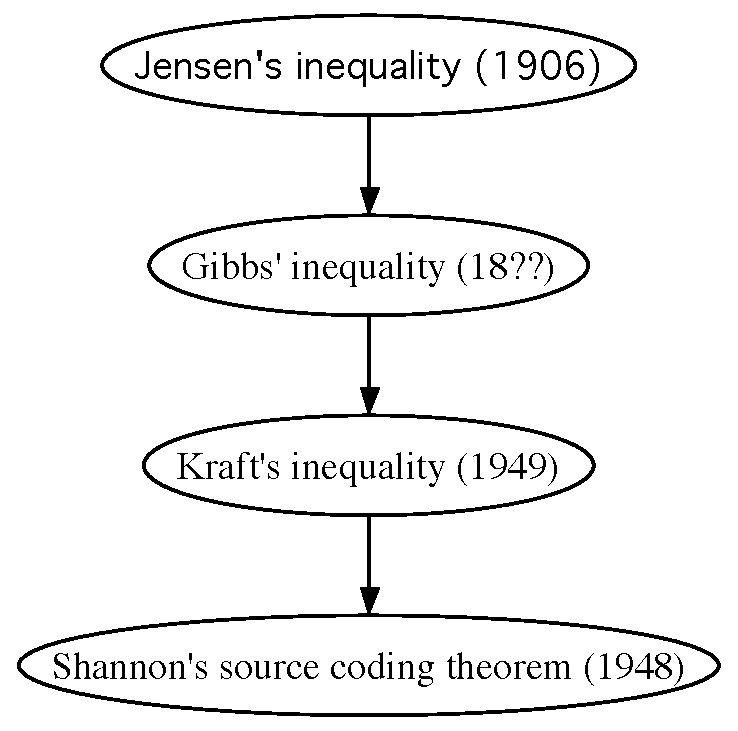
\includegraphics[height=.5\textheight]{theorems-dates.pdf} }

\itemb
\item Gibbs worked extensively on statistical mechanics. \alert{Where/when was Gibbs' inequality published?}
\item McMillan independently rediscovered Kraft's result in 1956.
\item Kraft \& McMillan cited (respectively) Redheffer \& Doob.
\item Shannon's formulation of his theorem was slightly different (asymptotic error rate of general block code).
\iteme

\end{frame}

\section{Practical Compression Schemes}

\begin{frame}{Huffman coding}

 \centerline{ 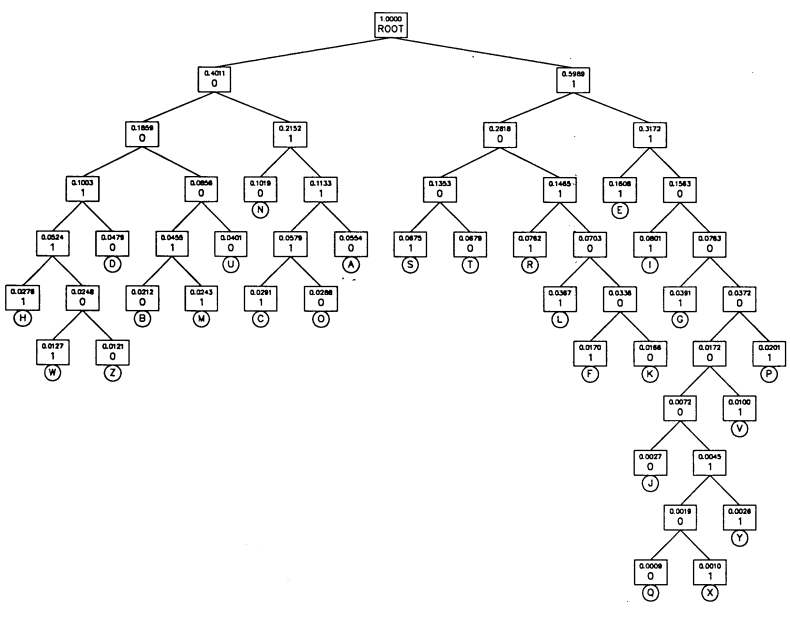
\includegraphics[height=.8\textheight]{huffman.png} }

\end{frame}

\begin{frame}{Huffman coding algorithm}

 \centerline{ 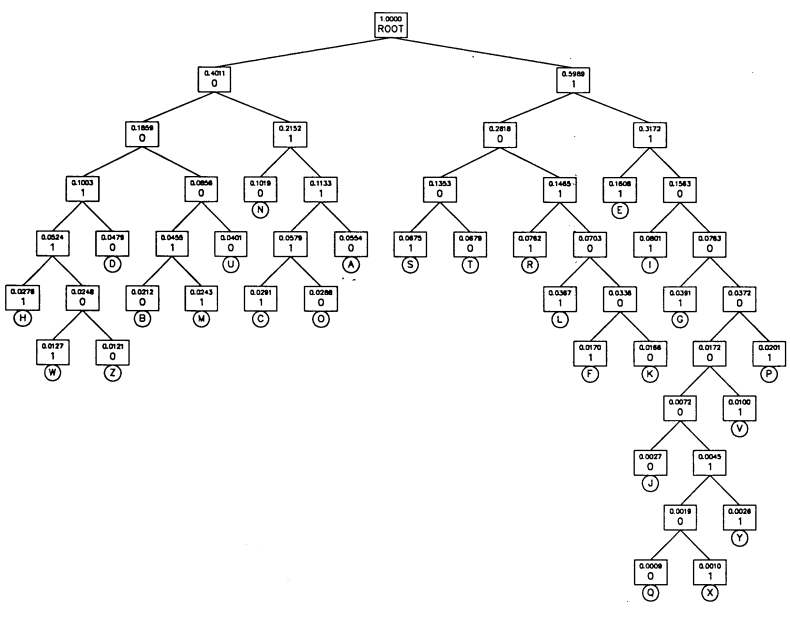
\includegraphics[height=.5\textheight]{huffman.png} }

\itemb
\item {\bf Huffman tree} generates optimal prefix codes with $L_p(C) < H_p + 1$ (but NB overhead of 1 bit/symbol).
 \inone{Bottom-up tree construction algorithm: combine the two least frequent symbols into a single symbol, and repeat.}
\iteme

\end{frame}

\begin{frame}{Arithmetic coding}

 \centerline{ 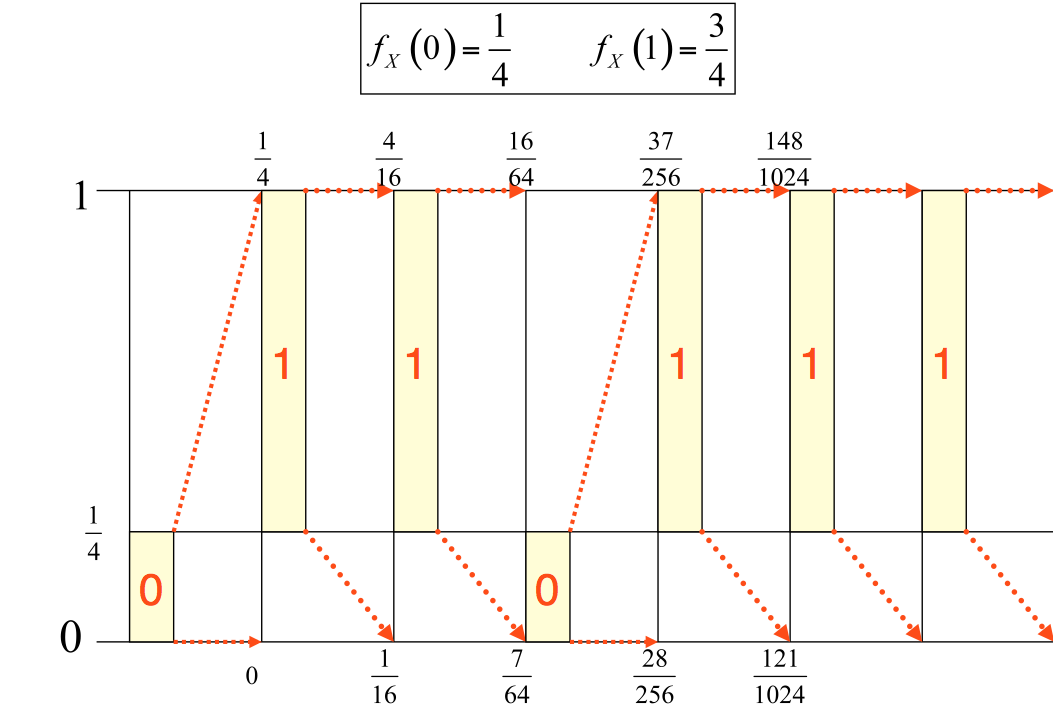
\includegraphics[height=.8\textheight]{Arithmetic_coding.png} }

\end{frame}

\begin{frame}{Arithmetic coding}
 \itemb
\item {\bf Arithmetic coding} is a block (not symbol) compression scheme that achieves asymptotically perfect efficiency.
\item The message ${\bf x}$ is represented as a subinterval of $[0,1)$
\itemb
 \item Subinterval found by recursive subdivision
 \item Width of subinterval $\simeq$ probability of message $P({\bf x})$
\iteme
\item Represent message as shortest binary fraction in subinterval
 \inone{Guaranteed to be expressible in $\sim -\log_2 P({\bf x})$ bits}
\iteme

\end{frame}


\begin{frame}{Arithmetic coding: the adaptive model}

\itemb
\item Represent the alphabet numerically: $\Omega = \{ 1, 2 \ldots N \}$
\item Suppose we have encoded $k-1$ characters of message ${\bf x}$
\item Let $k-1$'th interval be $[a,a+b)$
\item Next ($k$'th) interval is $[a',a'+b')$ where
\begin{eqnarray*}
a' & = & a + b \sum_{\omega=1}^{x_k - 1} p_k(\omega) \\
b' & = & b p_k(x_k) \\
p_k(\omega) & = & P(x_k = \omega | x_1 \ldots x_{k-1})
\end{eqnarray*}
\item Note that $p_k$ is \alert{adaptive} --- it has a ``memory'' of the last $k-1$ encoded/decoded characters
\iteme

\end{frame}

\begin{frame}{Arithmetic coding: issues}

\itemb
\item \alert{Underflow \#1:} finite precision
 \itemb
 \item Range delimiters $[a,b)$ may reach hardware precision limit
 \item Solution: while $a$ and $b$ have same top digit: output, shift, add padding digits
 \itemb
  \item e.g. $[.436,.437) \to [.600, .799)$ and output ``43''
  \item NB we pad $a$ with 0's and $b$ with 9's, to maximize range
 \iteme
 \iteme
\pause
\item \alert{Underflow \#2:} delimiters straddle boundary
 \itemb
 \item Decimal equivalent: ranges like [0.49999995,0.50000005)
 \item Top digits don't converge before underflow occurs
 \item Solution: extract next most significant digits, output them later (when top digits converge)
 \iteme
\pause
\item \alert{Floating-point math:} don't trust reproducibility of FPU
 \itemb
 \item No room for vagaries of floating-point math
 \item Solution: truncate all probabilities to some finite fraction
 \item Use integers throughout code (e.g. discretized log-probs)
 \iteme
\iteme

\end{frame}


\begin{frame}{Other symbol and number codes}

\itemb
\item Encoding symbols from finite alphabets
 \itemb
  \item \alert{Binary encoding}: use $k=\log_2 n$ bits to encode $n$ symbols
  \item \alert{Truncated binary encoding}: let $b = n - 2^k$.
  \itemb
   \item First $2^k - b$ symbols use first $2^k - b$ codewords of length $k$
   \item Remaining $2b$ symbols use {\bf last} codewords of length $k+1$
  \iteme
 \iteme
\item Encoding arbitrary integers, $n$
 \itemb
  \item \alert{Unary encoding}: transmit number $n$ as $n$ 1's, followed by a 0
  \item \alert{Golomb encoding}: choose parameter $m$
   \itemb
   \item transmit $n/m$ using unary encoding
   \item transmit $n\%m$ using truncated binary encoding
   \iteme
 \iteme
\iteme

Each of these is optimal for some probability distribution: \\
\alert{can you see which?}

\end{frame}

\begin{frame}{Codes based on repetition}

\itemb
\item Each of these has a shorthand for some repetition
\itemb
\item \alert{Run-length encoding}: repeated characters
\item Dictionary (\alert{Lempel-Ziv}) encoding: repeated words
 \itemb
  \item LZ77: sliding window
  \item LZ78: adaptive dictionary
 \iteme
\iteme
\item \alert{Which probability distribution is each optimal for?}
\inone{Imagine a process that generates such patterns....}
\iteme


\end{frame}

\begin{frame}{Probabilistic models used with arithmetic coding}

\itemb
\item ``Adaptive arithmetic coding'': updated frequency tables
\item Order-$N$ Markov chain
\item \alert{PPM}: Prediction by Partial Matching
\itemb
\item Attempts to predict using the previous $n$ characters
\item If previous $n$ not seen before, drops to $n-1$, then $n-2$, etc.
\item If no context seen, uses a flat (or, in PPMd, adaptive) prior
\iteme
\item \alert{PAQ}: uses a mixture of several prediction models
\itemb
\item PPM-like $n$-gram contexts
\inone{Various sparse and bit-twiddled subsets of such contexts}
\item Periodic contexts (period is heuristically estimated)
\item Customized models for specific file formats
\inone{.BMP, .TIFF. .JPEG, .EXE, etc.}
\iteme
\iteme

\end{frame}

\begin{frame}{Transformations of the input string}

\itemb
\item Idea: invertible operation, makes input easier to compress
\inone{e.g. aggregates disperse repetitions}
\item \alert{Burrows-Wheeler transform}, aka block-sorting
\itemb
 \item Sort all rotations of text, then take last column
 \inone{Invertible permutation of input string}
 \item Also has some excellent properties as a \alert{substring index}
\iteme
\item Turns repeated motifs $\leftrightarrow$ repeated characters
 \inone{Can then compress e.g. with run-length encoding or order-$N$ Markov}
\iteme


\end{frame}

\section{Compression of Biological Sequences}


\begin{frame}{Motivation: whole genome re-sequencing}

\itemb
\item Example: \alert{cancer re-sequencing} ({\bf International network of cancer genome projects}, ICGC, Nature 2010)
 \itemb
 \item At least 10 cancer resequencing projects by 2010 (many more coming)
 \item 300-500 samples per tumour
 \item Sequencing coverage at least 30X
 \item That's about $5 \times 10^{13}$ bases, per project
 \item FASTQ uses 8 bits for the base + 8 bits for the \alert{quality score}
 \item So, $10^{14}$ bytes $\simeq 60$ terabytes per project. OUCH
 \iteme
\item Could throw the data away after analysis.... unsatisfactory
\item \alert{Most of the reads are substrings of the reference genome}
\iteme

\end{frame}


\begin{frame}{Compression of reads to reference genome}

 \centerline{ 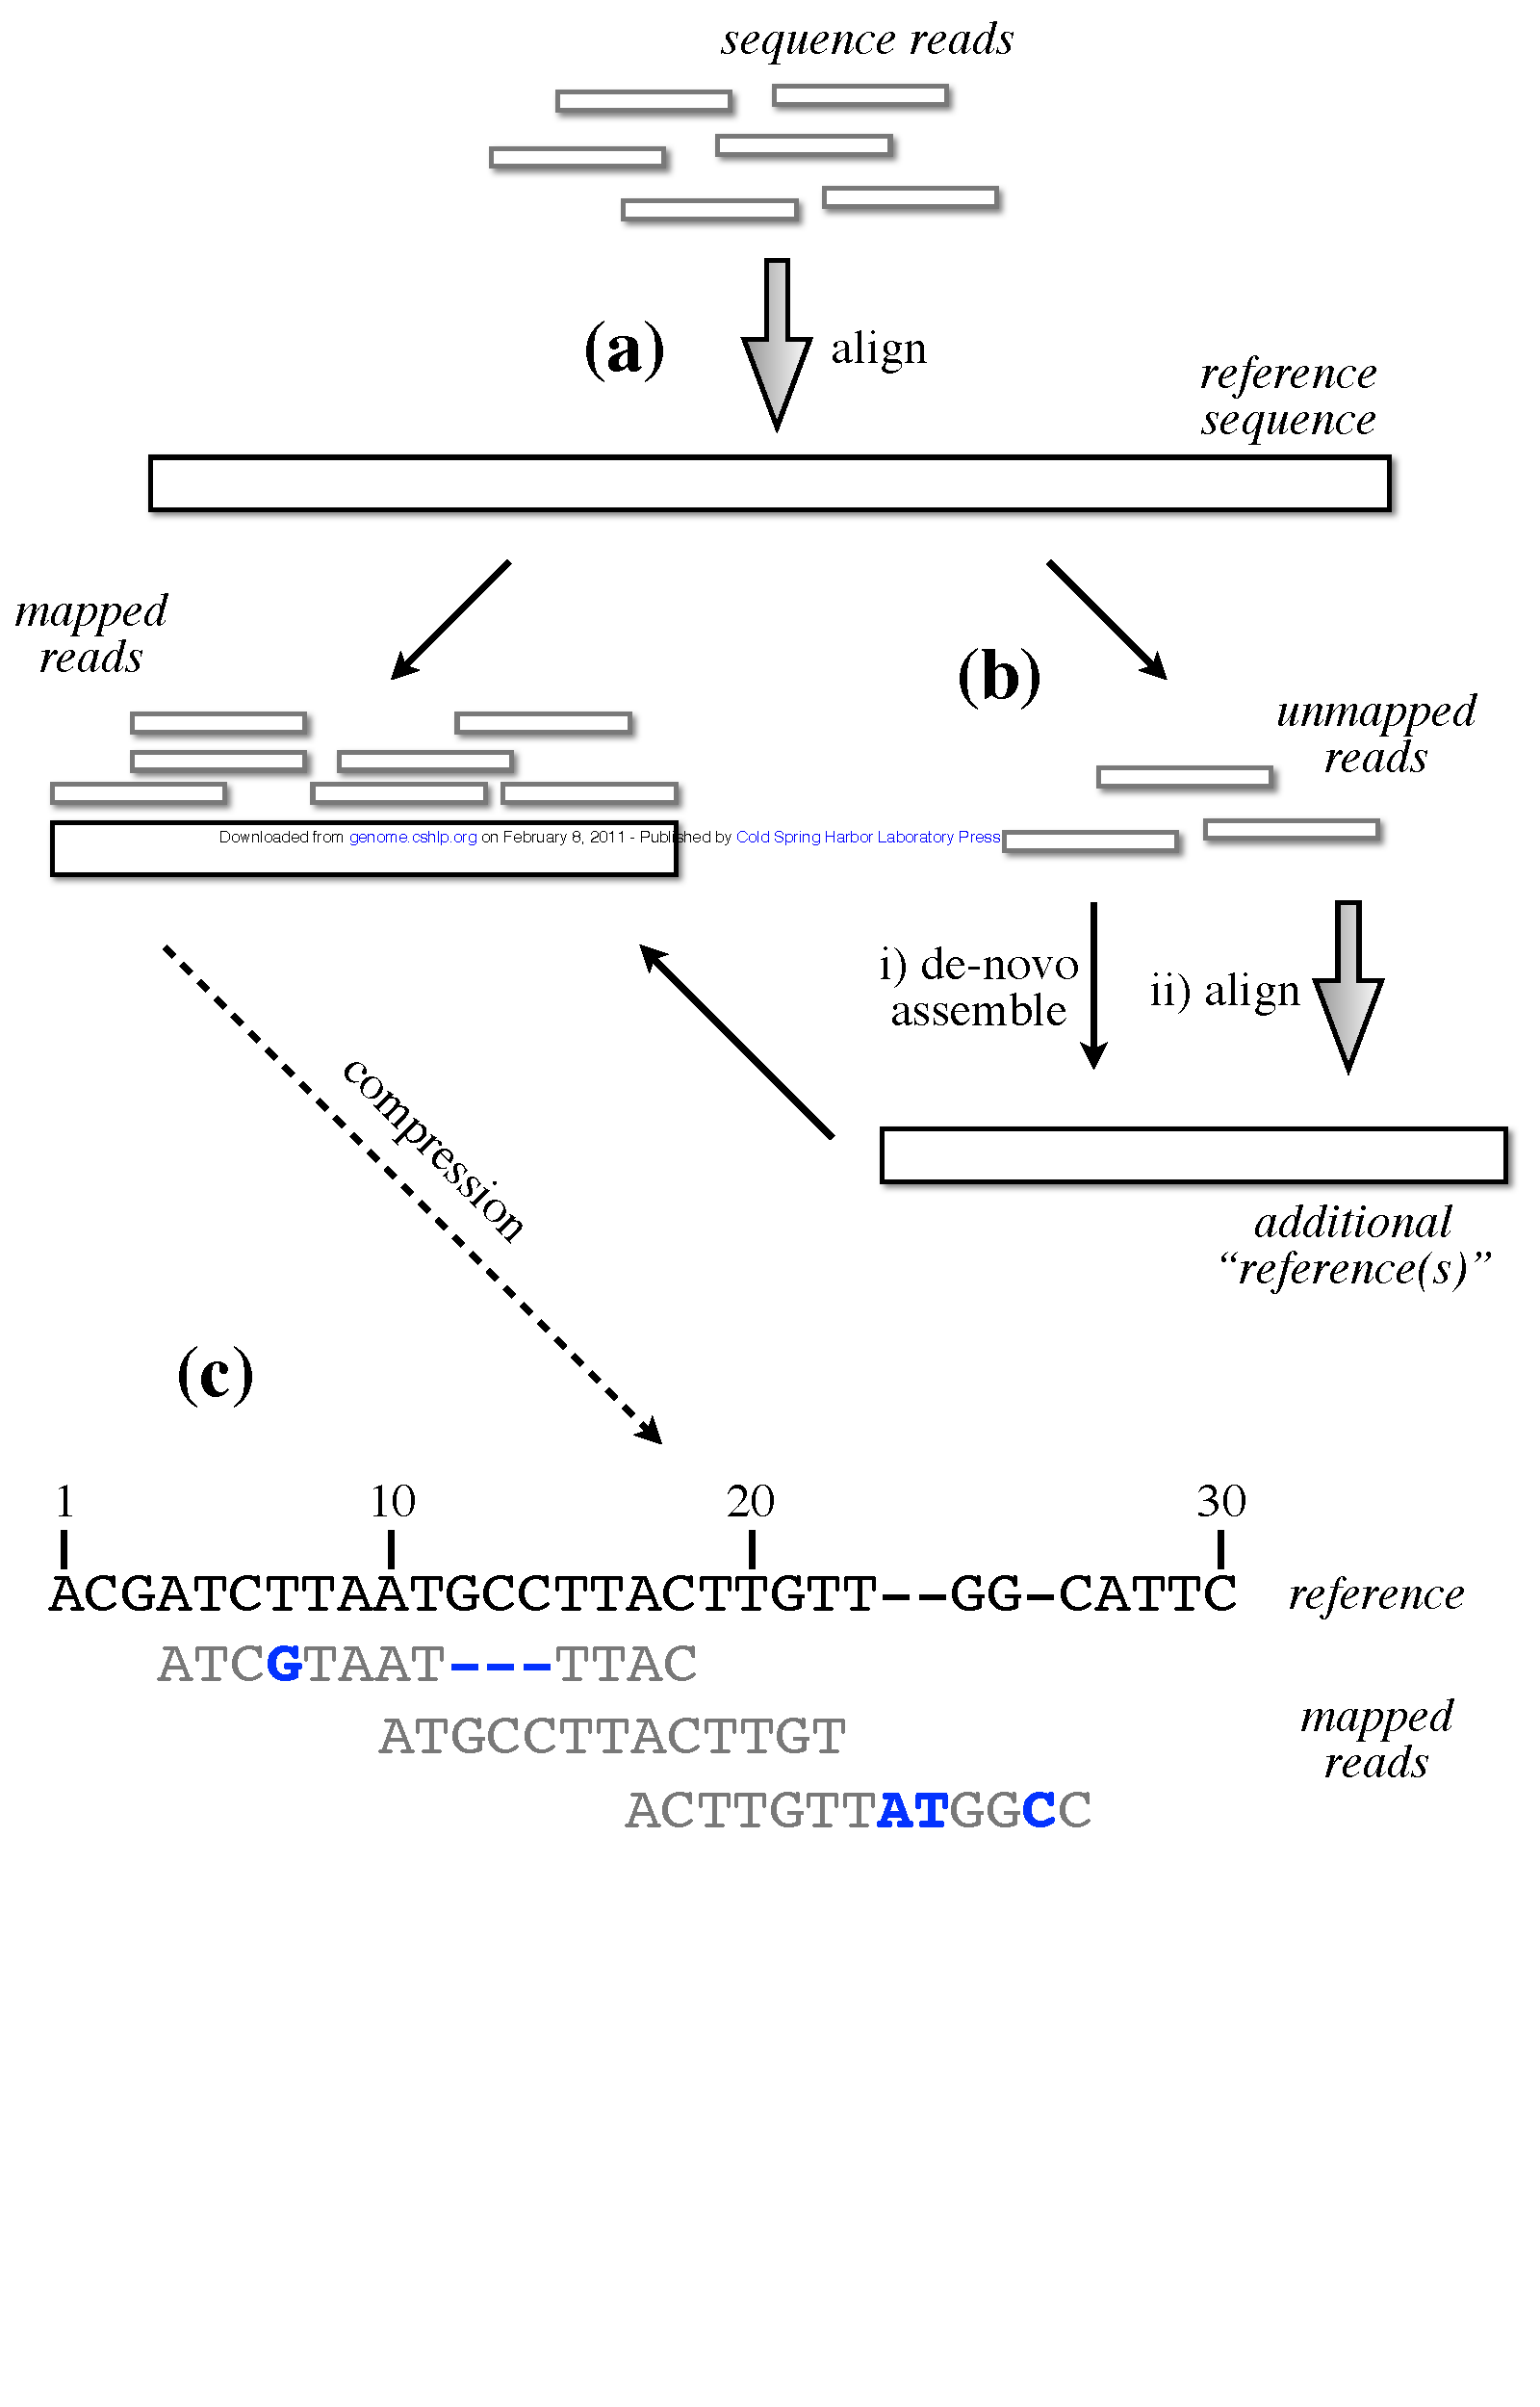
\includegraphics[height=.8\textheight]{BirneyEtAl.pdf} }
Birney {\em et al}. 2011.

\end{frame}


\begin{frame}{Compression of reads to reference genome}

\itemb
\item Central idea:
 \itemb
 \item \alert{Align reads to reference genome.}
 \inone{For unaligned reads, do \alert{{\em de novo} assembly}, then align to that}
 \item Store read lengths using \alert{Huffman coding.}
 \item Store distances between reads/differences using \alert{Golomb coding} ($m$ = expected distance between reads/differences)
 \item Read-pairs: use Golomb for separation, plus 3 extra bits to indicate strands \& relative orientation of paired reads.
 \item \alert{Lossy compression} of quality scores.
 \iteme
\item References:
\itemb
\item Birney {\em et al}.
{\bf Efficient storage of high throughput sequencing data using reference-based compression.}
Genome Research, 2011.
\item Baldi {\em et al}.
{\bf Data structures and compression algorithms for high-throughput sequencing technologies.}
BMC Bioinformatics, 2010.
\iteme
\iteme

\end{frame}


\begin{frame}{Underlying structure of Baldi/Birney methods}

\itemb
\item \alert{Augment} data before \alert{compressing} it.
\itemb
 \item Augmented data is easier to compress
\inone{e.g. as a delta from a known reference genome}
 \item Augmentation step involves (CPU-intensive) processing
 \item In this case augmentation = alignment (+ assembly)
 \item Could also imagine \alert{phylogenetic placement} as augmentation step
\iteme
\item Note that augmentation is theoretically unnecessary---we could marginalize the augmentation and shave off some bits---but this may be impractical, or even impossible due to complexity
\iteme

\end{frame}


\begin{frame}{Some other compression methods for genomes}

\itemb
\item NB these do not involve augmentation {\em or} short reads. Just ``straightforward'' compression of genomes
\itemb
\item Matsumoto {\em et al}, 2000. {\bf Biological sequence compression algorithms.} \alert{Finds repeats, palindromes; c.f. LZ77, LZ78}
\item Chen {\em et al}, 2002. {\bf DNACompress: fast and effective DNA sequence compression.} \alert{Finds repeats}
\item Christley {\em et al}, 2009. {\bf Human genomes as email attachments.} \alert{James Watson's genome in 4MB}
\iteme
\iteme

\end{frame}

\begin{frame}{The Right Way To Do It}

\itemb
\item Proposal: \alert{bio-oriented compression library}
\itemb
\item Arithmetic coding/decoding
\item Handlers for standard file formats
\item Preprocessing: assembly, alignment, annotation, phylogeny
\item Models: phylogenetic factor graphs, HMMs, SCFGs
\item Modular reference dictionaries that are themselves compressed
\iteme
\iteme

\end{frame}

\section*{Summary}

\begin{frame}{Summary}

  % Keep the summary *very short*.
  \begin{itemize}
  \item Compressed bits/symbol $\geq$ Shannon entropy/symbol
   \itemb
   \item Arithmetic coding approaches limit, given adaptive model:
\[
P(\mbox{next symbol}|\mbox{previous symbols})
\]
   \item Other codes (e.g. Golomb, Huffman, Lempel-Ziv) are easier to implement \& often run faster
   \item All codes have an implicit probability distribution for which they are ideal
   \iteme
 \item Transformation and preprocessing often useful
  \inone{e.g. aligning high-throughput sequence reads to reference genome}
 \end{itemize}

\end{frame}


\end{document}
